Deleted from ThesisCustom.sty

\newcommand{\nIp}[0]{\text{[nI\('\)]}}

\newcommand{\nIm}[0]{\text{[nIm]}}


% % % Paws % % %
\newcommand{\iDog}{%
  \mathrel{%
  
\begin{tikzpicture}
%    \tikz[line cap=round, line join=round]
    \draw[draw = white] (0,0) rectangle (0.3,0.3);
    \begin{scope}[overlay]
    \draw (0.15,.01) circle (2.25pt);
    \draw (0.15,.2) circle (1.125pt);
    \draw (0.05,.15) circle (1.125pt);
    \draw (0.25,.15) circle (1.125pt);
    \end{scope}
      \end{tikzpicture}
  }%
}

\newcommand{\iDogd}{%
  \mathrel{%
  
\begin{tikzpicture}
%    \tikz[line cap=round, line join=round]
    \draw[draw = white] (0,0) rectangle (0.3,0.3);
    \begin{scope}[overlay]
    \draw[dash pattern=on \pgflinewidth off .5pt] (0.15,.01) circle (2.25pt);
    \draw[dash pattern=on \pgflinewidth off .5pt] (0.15,.2) circle (1.125pt);
    \draw[dash pattern=on \pgflinewidth off .5pt] (0.05,.15) circle (1.125pt);
    \draw[dash pattern=on \pgflinewidth off .5pt] (0.25,.15) circle (1.125pt);
    \end{scope}
      \end{tikzpicture}
  }%
}

% % % Paws with backwards 'e' for pads % % %

\newcommand{\iEDogd}{%
  \mathrel{%
  
\begin{tikzpicture}
%    \tikz[line cap=round, line join=round]
    \draw[draw = white] (0,0) rectangle (0.3,0.3);
    \begin{scope}[overlay]
    %\draw[dash pattern=on \pgflinewidth off .5pt] (0.15,.01) circle (2.25pt);
    \node[scale=0.9] (1,0.1) [label={[xshift=0.155cm, yshift=-.3125cm]\reflectbox{\textsf{e}}}] {};
    \draw[dash pattern=on \pgflinewidth off .5pt] (0.15,.2) circle (1.125pt);
    \draw[dash pattern=on \pgflinewidth off .5pt] (0.05,.15) circle (1.125pt);
    \draw[dash pattern=on \pgflinewidth off .5pt] (0.25,.15) circle (1.125pt);
    \end{scope}
      \end{tikzpicture}
  }%
}

\newcommand{\iEDog}{%
  \mathrel{%
  
\begin{tikzpicture}
%    \tikz[line cap=round, line join=round]
    \draw[draw = white] (0,0) rectangle (0.3,0.3);
    \begin{scope}[overlay]
    %\draw[dash pattern=on \pgflinewidth off .5pt] (0.15,.01) circle (2.25pt);
    \node[scale=0.9] (1,0.1) [label={[xshift=0.155cm, yshift=-.3125cm]\reflectbox{\textsf{e}}}] {};
    \draw (0.15,.2) circle (1.125pt);
    \draw (0.05,.15) circle (1.125pt);
    \draw (0.25,.15) circle (1.125pt);
    \end{scope}
      \end{tikzpicture}
  }%
}

\newcommand{\nr}[0]{\emph{non utendo referat}} % de constructione
\newcommand{\ur}[0]{\emph{utendo referat}} % de materia

\newcommand{\mcA}[0]{Conditional A}
\newcommand{\mcB}[0]{Conditional B}


% % % % % % % % % % % % % % % % % % % % % % % % % % % % % % % % % % %
% A collection of commands to ensure that the contents of nI/LCS are always the same when repeated.
\newcommand{\nIClauseClaimedSupport}{%
  \obeybreaks{\(S\) performed some reasoning which culminated with \(\phi\) having value \(v\), though remains epistemic possibility that \(\phi\) does not have value \(v\).}% from materia \(M\) and continues to claim support for \(\phi\) having value \(v\) from materia \(M\).}%
}
\newcommand{\nIClausePsiIsNew}{%
  \obeybreaks{{\color{red} \(S\) did not have information about \(\psi\) when claiming support for \(\phi\).}}%
}
% \newcommand{\nIClauseReceivedInfo}{%
%   \obeybreaks{\(S\) has claimed support that if \(\phi\) has value \(v\) then \(\psi\) has value \(v'\).}%
% }
\newcommand{\nIClauseInclusion}{%
  \obeybreaks{\(S\) is confident that:}%
}
\newcommand{\nIClauseInclusionPosition}{%
  \obeybreaks{If \(S\)' reasoning for \(\phi\) having value \(v\) is \nmom{} then \(S\) is, given present context, in a position to reason to \(\psi\) having value \(v'\) (without appealing to prior reasoning for \(\phi\) having value \(v\)).}%
}
\newcommand{\nIClauseInclusioBound}{%
  \obeybreaks{If \(S\)' reasoning for \(\phi\) having value \(v\) is \nmom{} then \(S\) would not be \mom{} were \(S\) to reason to \(\psi\) having value \(v'\).}%
}
\newcommand{\nIClauseValue}{%
  \obeybreaks{Reasoning is such that:}%
}
\newcommand{\nIClauseValuePhi}{%
  \obeybreaks{The reasoning appeals to \(\phi\) having value \(v\) as a premise, such that \(\phi\) having value \(v\) is obtained from the reasoning that \(\phi\) has value \(v\) noted in~\ref{nI:background}, and fail without the move}%
}
\newcommand{\nIClauseValuePsi}{%
  \obeybreaks{\(\psi\) only successful if \(\phi\).}%
}


% % % %
\ExplSyntaxOn
\DeclareDocumentCommand{\RIPa}{ m }{% No inertia
  \tl_if_empty:nTF {#1}
  {
    \text{big}%
  }
  {%
    \text{Big}%
  }
}
\ExplSyntaxOff

\ExplSyntaxOn
\DeclareDocumentCommand{\RIPb}{ m }{% No inertia
  \tl_if_empty:nTF {#1}
  {
    \text{playful}%
  }
  {%
    \text{Playful}%
  }
}
\ExplSyntaxOff


\newcommand{\sinkSymb}{%
  \mathrel{%
  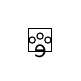
\begin{tikzpicture}

    \draw (0,0) rectangle (0.3,0.3);
    \begin{scope}[overlay]

    \node[scale=0.9] (1,0.1) [label={[xshift=0.155cm, yshift=-.3125cm]\reflectbox{\textsf{e}}}] {};
    \draw (0.15,.2) circle (1.125pt);
    \draw (0.05,.15) circle (1.125pt);
    \draw (0.25,.15) circle (1.125pt);
    \end{scope}
      \end{tikzpicture}
  }%
}